\section{Results}
This section contains the results obtained during the design of the three units of the project.
\subsection{Discharge Flow Control Unit}
\subsubsection{Flow control sub-unit}
An MG996R servo motor was selected for this sub-unit, to open and close the valve in steps that can be less than $1^{0}$ depending on the number of steps requested by the user. Direct pulse width modulation was preferred to a micro-step drive as a mechanism to drive the servo motor in steps of any size.
\par
A mounting mechanism for the servo motor was designed to the specs of the motor and stress-tested. It was found to withstand the maximum torque of the motor.   
\subsubsection{Flow diversion sub-unit}
A P16-S micro-linear actuator with a linear stroke length of 100mm and stroke-speed of 150mm/s was selected to operate a flap used to divert the discharge flow either into the main reservoir or the discharge collection tank.
\par 
 A four-bar kinematic chain was designed and simulated in MechDesigner based on the motion required for the flap. The chain achieved the motion based on the cam data obtained from the simulation.
\par
\subsubsection{Unit Assembly}
The assembly of the discharge flow control unit is shown in figure \ref{fig:unit_exploded_view}.
\begin{figure}[H]
    \centering
    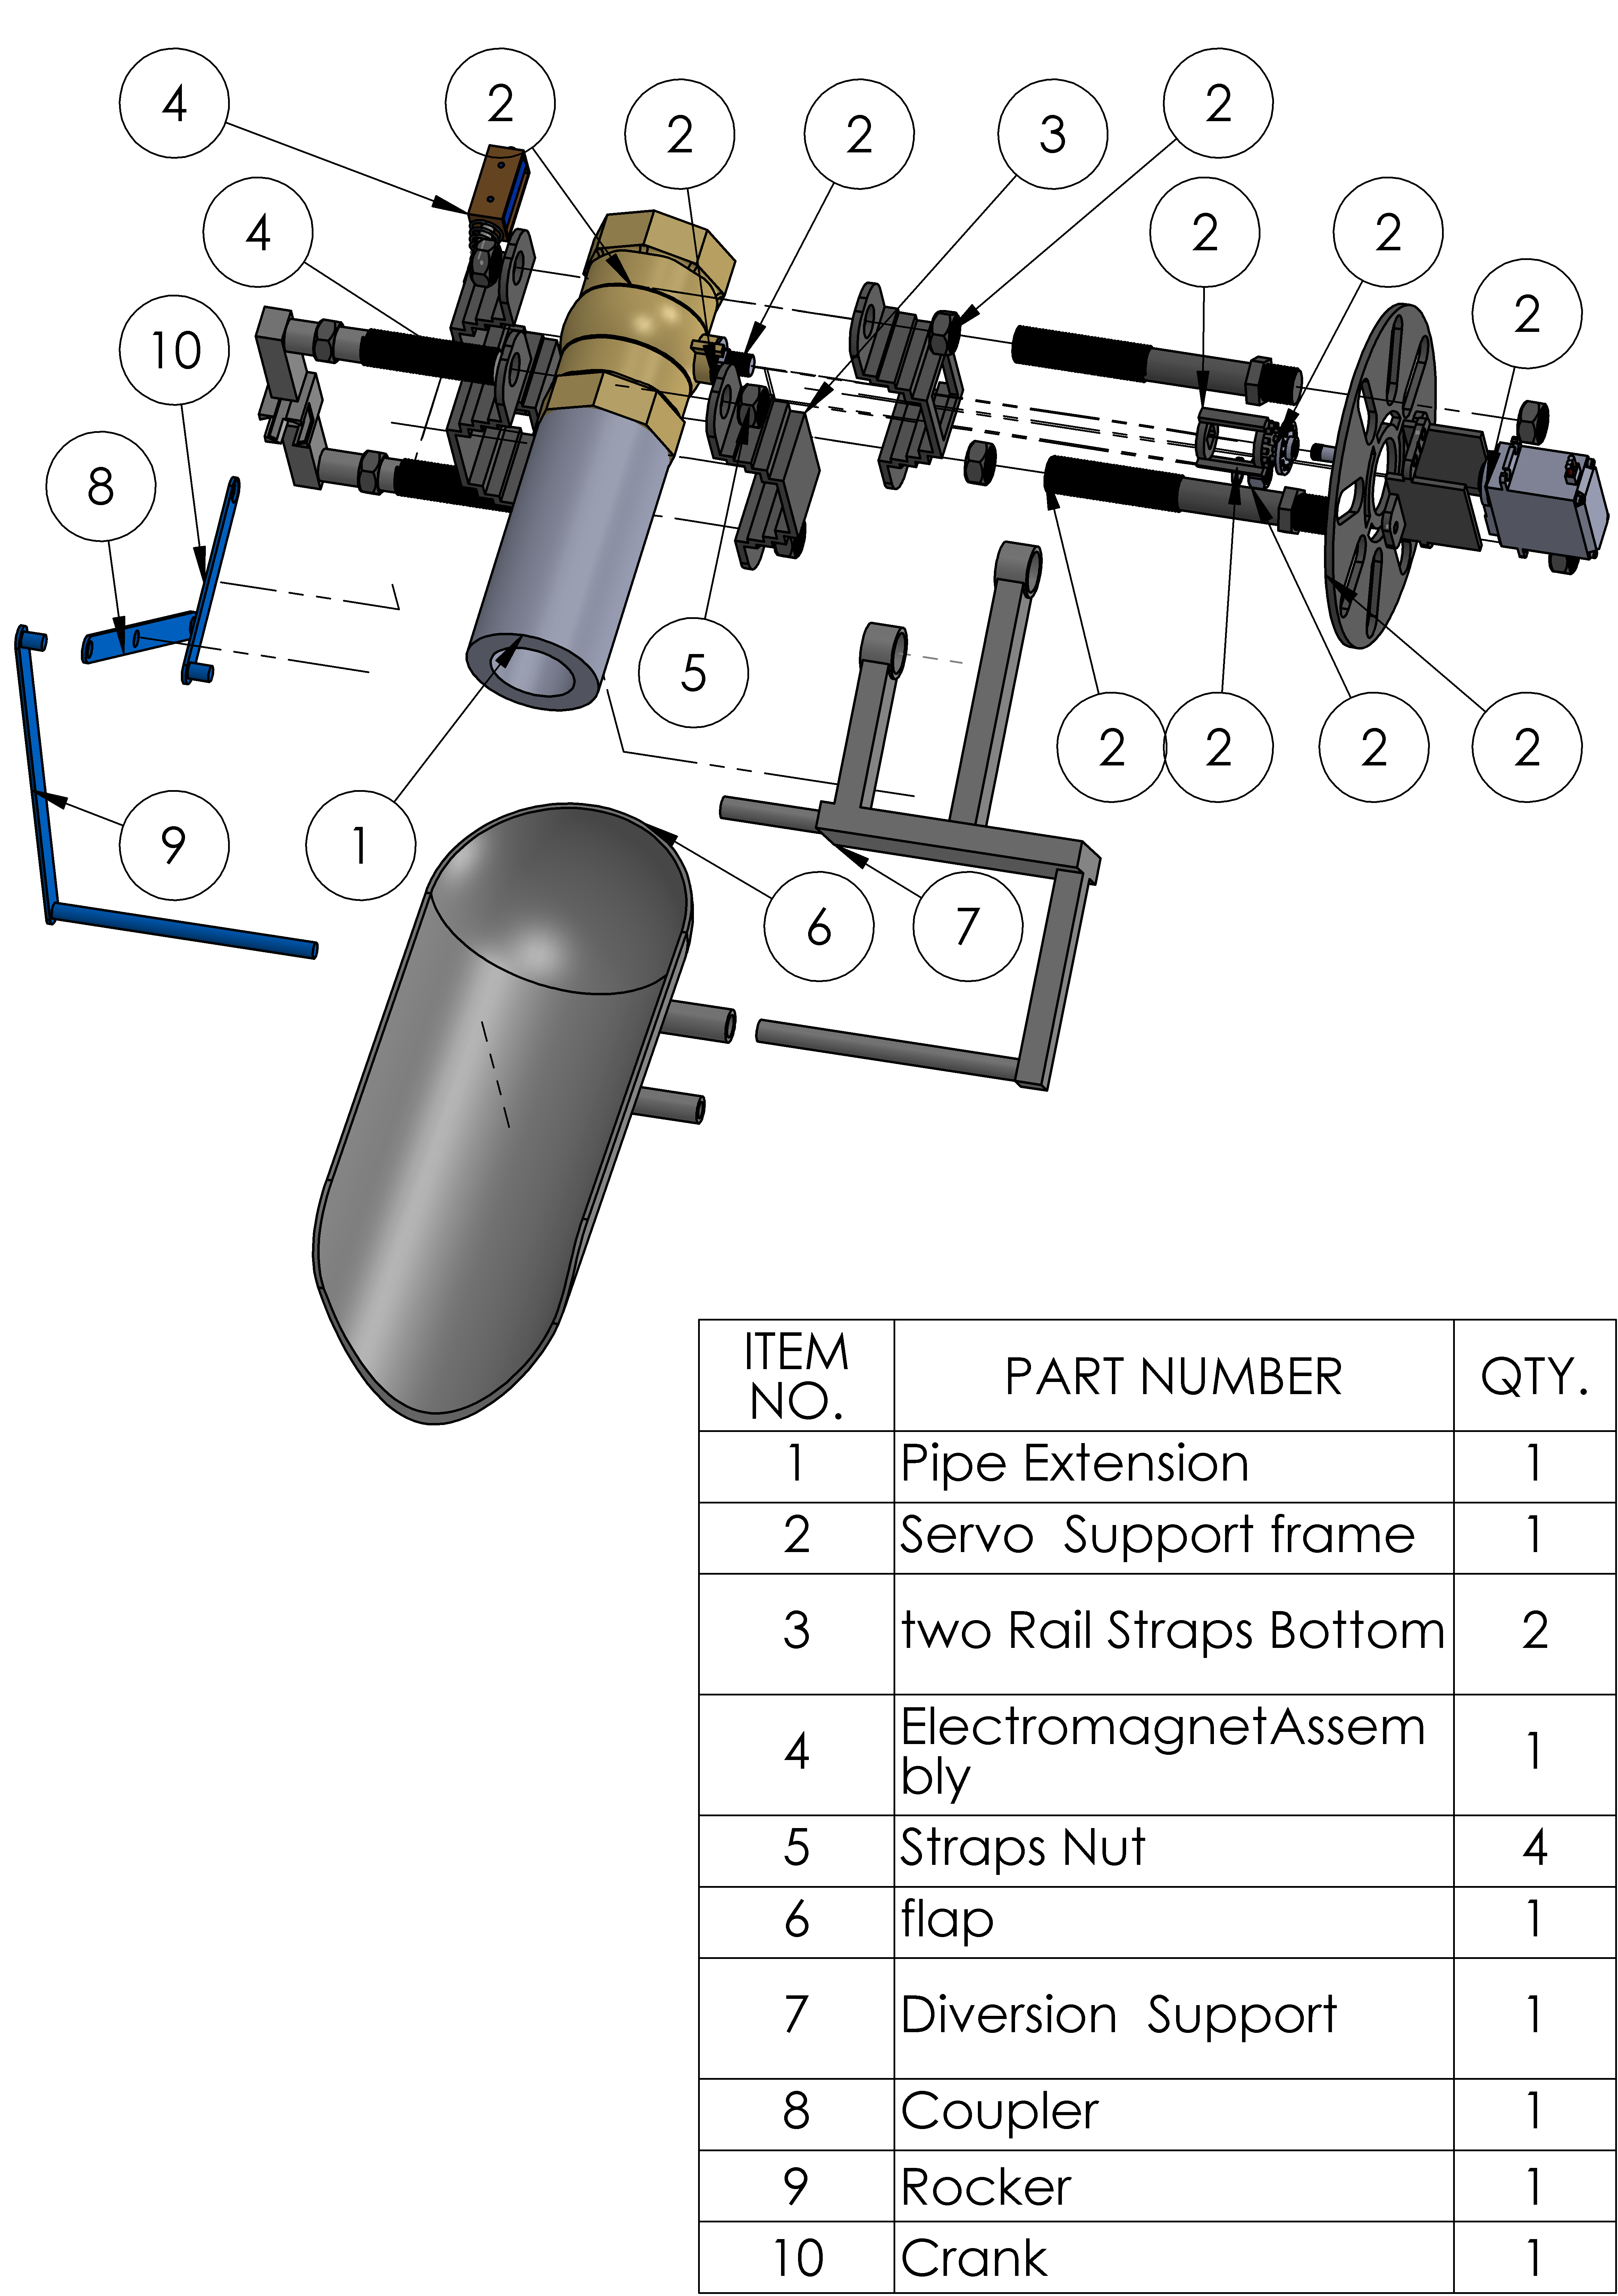
\includegraphics{Figures/DischargeFlowDiverSionAssembly5.PNG}
    \caption{Unit Exploded view}
    \label{fig:unit_exploded_view}
\end{figure}
From a motion study simulation in SolidWorks, the assembly appears to be able to regulate the fluid flow in steps as per the users specifications. The diversion unit also seems to be able to divert the flow either to the main reservoir or to the discharge collection tank.

\subsection{Discharge Flow Handling unit}
\subsubsection{Discharge collection tank sub-unit}
A horizontal half-cylindrical tank was preferred to a cuboid tank from a simulation that showed that the pressure of the collected fluid will concentrate on a line at the bottom of the tank. This is preferred in this application in order to minimize the time taken to empty the tank.
\subsubsection{Outlet valve sub-unit}
A solenoid valve was preferred to a butterfly valve because of its relatively cheaper price though the preferred size is slower.
\subsubsection{Weight measurement sub-unit}
Four load cells connected on a Wheatstone bridge were preferred to an ultrasonic approach to measure the weight of the collected discharge because the ultrasonic approach is unreliable.
\subsubsection{Temperature measurement sub-unit}
A DS18B20 immersible temperature sensor was selected for this subunit due to its reliability and sensitivity.
\par
\subsubsection{Final assembly}
Figure \ref{fig:final assembly} shows the designed system attached to the Synthetic Hydro-Experimental Machine currently in use in JKUAT.
\begin{figure}[H]
    \centering
    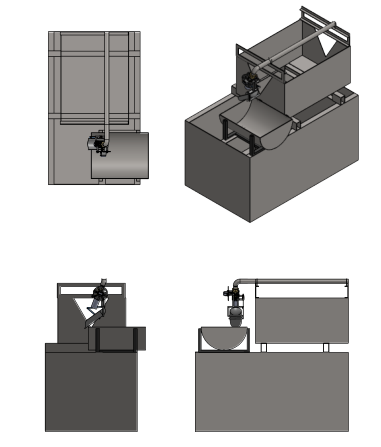
\includegraphics[width=\textwidth,height=0.75\textheight,keepaspectratio]{Figures/final assembly.png}
    \caption{Final Assembly}
    \label{fig:final assembly}
\end{figure}
 The dimensions of the part are derived from the existing machine.
 
\subsection{Budget}
The table \ref{tab:budget} shows the budget of the project.
\begin{table}[H]
\centering
\resizebox{\columnwidth}{!}{%
\begin{tabular}{|l|l|l|l|l|l|}
\hline
\textbf{Item No.} & \textbf{Item} & \textbf{Description} & \textbf{Unit Cost} & \textbf{No.} & \textbf{Total Cost} \\ \hline
1 & Servo Motor & MG996R(4.8Kg/cm) & 800 & 1 & 800 \\ \hline
2 & Linear Actuator & P16-S Linear Actuator & 3500 & 1 & 3500 \\ \hline
3 & Load cells & 50 Kg Load cells & 150 & 4 & 600 \\ \hline
4 & Load cell Amplifier & HX711 & 100 & 1 & 100 \\ \hline
5 & Temperature Sensor & DS18B20 Immersible & 300 & 1 & 300 \\ \hline
6 & Solenoid valve & 3/4''  Plastic & 900 & 1 & 900 \\ \hline
7 & MCU & STM32F407VET6 & 4400 & 1 & 4400 \\ \hline
8 & LCD & 320x240 Touch LCD & 1200 & 1 & 1200 \\ \hline
9 & Power MOSFET & IRF520 N-ch & 550 & 3 & 1650 \\ \hline
10 & Voltage Regulator & XL4015 DC-DC adjustable buck module & 400 & 3 & 1200 \\ \hline
11 & Transformer & AC 220V TO DC 12V 5A Transformer Power Supply & 1100 & 1 & 1100 \\ \hline
12 & Fabrication Cost & 3D printing \& Others & 10000 & 1 & 10000 \\ \hline
Total &  &  &  &  & \textbf{22600} \\ \hline
\end{tabular}%
}
\caption{Budget}
\label{tab:budget}
\end{table}

\begin{itemize}
    \item \textbf{Shipping}\\
    Some of the components such as P16-s micro-linear actuator, and the MCU with LCD,  are not available locally. The price indicated in the budget has their shipping cost included.
    \item \textbf{Good deals}\\
    Components such as strain-type load cells goes for Ksh. 250 a piece in Kenya. The four of them would have been Ksh. 1000 plus the amplifier, Ksh. 1100. A temporary good deal was found on AliExpress, that reduced the price by half. The same case applied to the MCU board with the LCD.
    \item \textbf{Fabrication cost}\\
    The fabrication cost indicated in the budget is the maximum possible estimate. Since most of the materials will be provided in the school's workshops, this cost might reduce. 
\end{itemize}


